% begin module EVT-hypotheses
\begin{frame}[t]
\begin{theorem}[The Extreme Value Theorem]
If \alert<3-4>{$f$ is continuous} on a \alert<5-6>{closed interval $[a,b]$}, then $f$ attains its maximum and minimum value, each at least once.
\end{theorem}
\begin{columns}[c]
\column{.5\textwidth}
\ \uncover<3->{%
\psset{xunit=0.7cm, yunit=0.7cm}
\begin{pspicture}(-0.5,-1.5)(7,4)
\psframe*[linecolor=white](-0.5,-1.5)(7,4)
\psaxes[ticks=none, labels=none]{<->}(0,0)(-0.5,-1.5)(7,4)\tiny
\psLabels{7}{4}
\psXTick{1}
\rput[t](1, -0.2){$a$}
\psXTick{6}
\rput[t](6, -0.2){$b$}
\psFullDot{1}{2.75}
\psFullDot{6}{2}
\psHollowDot{4}{-1}
\psFullDot{4}{1}
%Function formula: 2- ((-3+1/2 (x))^{2}) 
\psplot[linecolor=red, plotpoints=1000]{4}{6}{x 0.5 mul -3 add 2 exp -1 mul 2 add } %Function formula: 3- ((1/2 (x))^{2}) 
\psplot[linecolor=red, plotpoints=1000]{1}{4}{x 0.5 mul 2 exp -1 mul 3 add }
\end{pspicture} 
%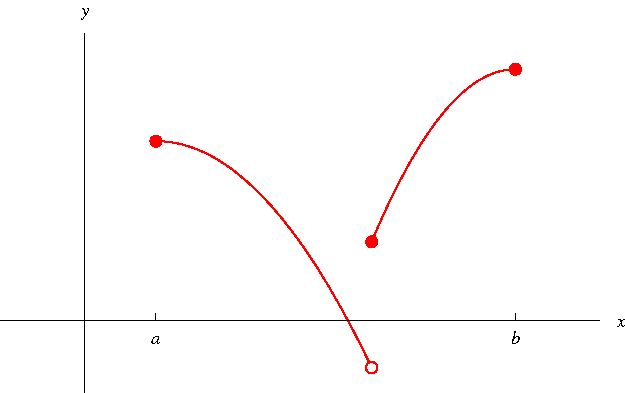
\includegraphics[width=6cm]{maxima-minima/pictures/04-01-evtcounterb.pdf}%
}%
\column{.5\textwidth}
\ \uncover<5->{%
\psset{xunit=0.7cm, yunit=0.7cm}
\begin{pspicture}(-0.5,-1.5)(7,4)
\psframe*[linecolor=white](-0.5,-1.5)(7,4)
\tiny
\psaxes[ticks=none, labels=none]{<->}(0,0)(-0.5,-1.5)(7,4)
\psLabels{7}{4}
\psXTick{1}
\rput[t](1, -0.2){$a$}
\psXTick{6}
\rput[t](6, -0.2){$b$}
\psHollowDot{1}{0.447214}
\psline[linestyle=dashed](6, 0)(6,4)
%Function formula: (1)/((6- (x))^{1/2}) 
\psplot[linecolor=red, plotpoints=1000]{1}{5.93}{1 x -1 mul 6 add 0.5 exp div }
\end{pspicture} 
%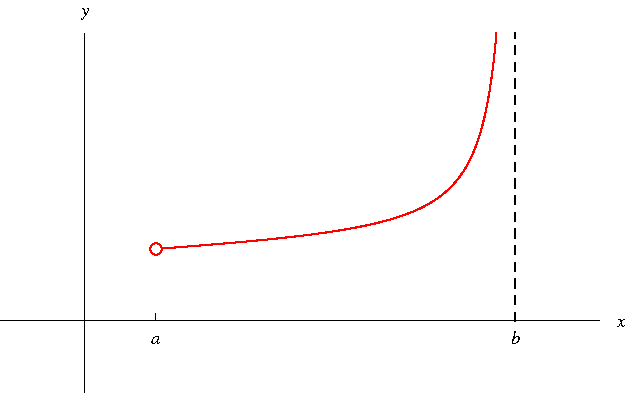
\includegraphics[width=6cm]{maxima-minima/pictures/04-01-evtcountera.pdf}%
}%
\end{columns}
\begin{itemize}
\item  Do we need all of the hypotheses of the theorem?
\item<2-| alert@3-4>  Do we need $f$ to be continuous?  \uncover<4->{Yes.}
\item<2-| alert@5-6>  Do we need the interval to be closed?  \uncover<6->{Yes.}
\end{itemize}
\end{frame}
% end module EVT-hypotheses
